%
% The first command in your LaTeX source must be the \documentclass command.
\documentclass[sigconf]{acmart}
%\documentclass{acmart}

%
% defining the \BibTeX command - from Oren Patashnik's original BibTeX documentation.
\def\BibTeX{{\rm B\kern-.05em{\sc i\kern-.025em b}\kern-.08emT\kern-.1667em\lower.7ex\hbox{E}\kern-.125emX}}
    
% Rights management information. 
% This information is sent to you when you complete the rights form.
% These commands have SAMPLE values in them; it is your responsibility as an author to replace
% the commands and values with those provided to you when you complete the rights form.
%
% These commands are for a PROCEEDINGS abstract or paper.
%\copyrightyear{2018}
%\acmYear{2018}
%\setcopyright{acmlicensed}
%\acmConference[Woodstock '18]{Woodstock '18: ACM Symposium on Neural Gaze Detection}{June 03--05, 2018}{Woodstock, NY}
% \acmBooktitle{Woodstock '18: ACM Symposium on Neural Gaze Detection, June 03--05, 2018, Woodstock, NY}
% \acmPrice{15.00}
% \acmDOI{10.1145/1122445.1122456}
% \acmISBN{978-1-4503-9999-9/18/06}

%
% These commands are for a JOURNAL article.
%\setcopyright{acmcopyright}
%\acmJournal{TOG}
%\acmYear{2018}\acmVolume{37}\acmNumber{4}\acmArticle{111}\acmMonth{8}
%\acmDOI{10.1145/1122445.1122456}

%
% Submission ID. 
% Use this when submitting an article to a sponsored event. You'll receive a unique submission ID from the organizers
% of the event, and this ID should be used as the parameter to this command.
%\acmSubmissionID{123-A56-BU3}

%
% The majority of ACM publications use numbered citations and references. If you are preparing content for an event
% sponsored by ACM SIGGRAPH, you must use the "author year" style of citations and references. Uncommenting
% the next command will enable that style.
%\citestyle{acmauthoryear}

%
% end of the preamble, start of the body of the document source.
\begin{document}

%\bibliography{/Users/ClayElmore/Desktop/mendeley/DMD_Literature.bib}

%
% The "title" command has an optional parameter, allowing the author to define a "short title" to be used in page headers.
\title{Stochastic Energy Market Price Forecasting with Recurrent Neural Networks}

%
% The "author" command and its associated commands are used to define the authors and their affiliations.
% Of note is the shared affiliation of the first two authors, and the "authornote" and "authornotemark" commands
% used to denote shared contribution to the research.

\author{Elmore, Clay}
%\authornote{Both authors contributed equally to this research.}
\email{celmore1@nd.edu}
\affiliation{%
  \institution{University of Notre Dame}
}

\author{Kopp, Grace}
\email{gkopp@nd.edu}
\affiliation{%
  \institution{University of Notre Dame}
}
%
% By default, the full list of authors will be used in the page headers. Often, this list is too long, and will overlap
% other information printed in the page headers. This command allows the author to define a more concise list
% of authors' names for this purpose.
\renewcommand{\shortauthors}{Elmore and Kopp, et al.}

% ============================================================================================================================= %
%														Abstract																       %
% ============================================================================================================================= %

\begin{abstract}
This project proposes to construct a neural network that will forecast energy prices in the California Independent System Operator (CAISO). Accurate forecasting of energy prices in the CISO provides an economic opportunity for energy providers to incur profit and buyers to purchase at the lowest possible price. Traditional methods for forecasting have been used for many years to forecast these prices, but the recent advances in recurrent neural network time series forecasting presents a possible way to improve upon existing methods. The problem statement of this project is how to design a neural network to accurately predict stochastic energy prices.
\end{abstract}

%
% The code below is generated by the tool at http://dl.acm.org/ccs.cfm.
% Please copy and paste the code instead of the example below.
%
% \begin{CCSXML}
% <ccs2012>
%  <concept>
%   <concept_id>10010520.10010553.10010562</concept_id>
%   <concept_desc>Computer systems organization~Embedded systems</concept_desc>
%   <concept_significance>500</concept_significance>
%  </concept>
%  <concept>
%   <concept_id>10010520.10010575.10010755</concept_id>
%   <concept_desc>Computer systems organization~Redundancy</concept_desc>
%   <concept_significance>300</concept_significance>
%  </concept>
%  <concept>
%   <concept_id>10010520.10010553.10010554</concept_id>
%   <concept_desc>Computer systems organization~Robotics</concept_desc>
%   <concept_significance>100</concept_significance>
%  </concept>
%  <concept>
%   <concept_id>10003033.10003083.10003095</concept_id>
%   <concept_desc>Networks~Network reliability</concept_desc>
%   <concept_significance>100</concept_significance>
%  </concept>
% </ccs2012>
% \end{CCSXML}

% \ccsdesc[500]{Computer systems organization~Embedded systems}
% \ccsdesc[300]{Computer systems organization~Redundancy}
% \ccsdesc{Computer systems organization~Robotics}
% \ccsdesc[100]{Networks~Network reliability}

%
% Keywords. The author(s) should pick words that accurately describe the work being
% presented. Separate the keywords with commas.
\keywords{machine learning, stochastic forecasting, recurrent neural networks, energy markets}

%
% A "teaser" image appears between the author and affiliation information and the body 
% of the document, and typically spans the page. 
% \begin{teaserfigure}
%   \includegraphics[width=\textwidth]{sampleteaser}
%   \caption{Seattle Mariners at Spring Training, 2010.}
%   \Description{Enjoying the baseball game from the third-base seats. Ichiro Suzuki preparing to bat.}
%   \label{fig:teaser}
% \end{teaserfigure}

%
% This command processes the author and affiliation and title information and builds
% the first part of the formatted document.
\maketitle

% ============================================================================================================================= %
%														Intro  																       %
% ============================================================================================================================= %

\section{Introduction}
\label{sec:intro}

Energy markets are present all around the globe. Prices in these markets are extremely volatile due to a variety of different factors including but limited to market demand, erratic weather, natural resource availability, and so much more. Because of the large swings in these prices, participating in these energy markets presents an economic opportunity to both energy buyers and sellers alike. For an energy provider, knowing when the price of energy will be high is critical to knowing when to use valuable resources to produce energy. For an energy user, knowing when to buy energy on the market at a low price can be the difference between an industrial user being profitable or going under. With these considerations in mind, it is clear that energy price forecasting is a worthy venture for academics to study because of its direct applicability to the commercial world.\\

In this paper, we will explore a specific energy market: the California Independent System Operator (CAISO). The CAISO is an enormous, complex energy market system in which energy buyers and sellers schedule a multitude of energy related transactions. The CAISO had some 40 billion dollars in sales, and more than 260,000 gigawatts sold in 2015\cite{CAenergy2}. This complex system makes for a data-rich problem worthy for study by academics and industry professionals alike. A particularly interesting problem in the CAISO is the forecasting of Day-Ahead Market (DAM) prices which are notoriously stochastic. DAM prices are used to forecast energy prices a day in advance which energy buyers and sellers then use to schedule when they will buy and sell energy on the CAISO market. It has been shown that accurate forecasting is absolutely critical to profiting off DAM market prices\cite{Dowling2017}.\\

Although prices in the CAISO DAM are quite volatile, they have very clear periodic tendencies. Figure \ref{fig:ex_prices} shows an example week of energy prices for an energy resource in the CAISO DAM for the first week of 2015. Note how the price is clearly periodic, but also has stochastic tendencies as well. Furthermore, Figure \ref{fig:ex_prices} shows the economic opportunity available to sell at high prices and buy at low prices. Some price swings are almost double the price. An accurate forecast would allow for large amounts of profit to be extracted from these systems.\\

\begin{figure}[h]
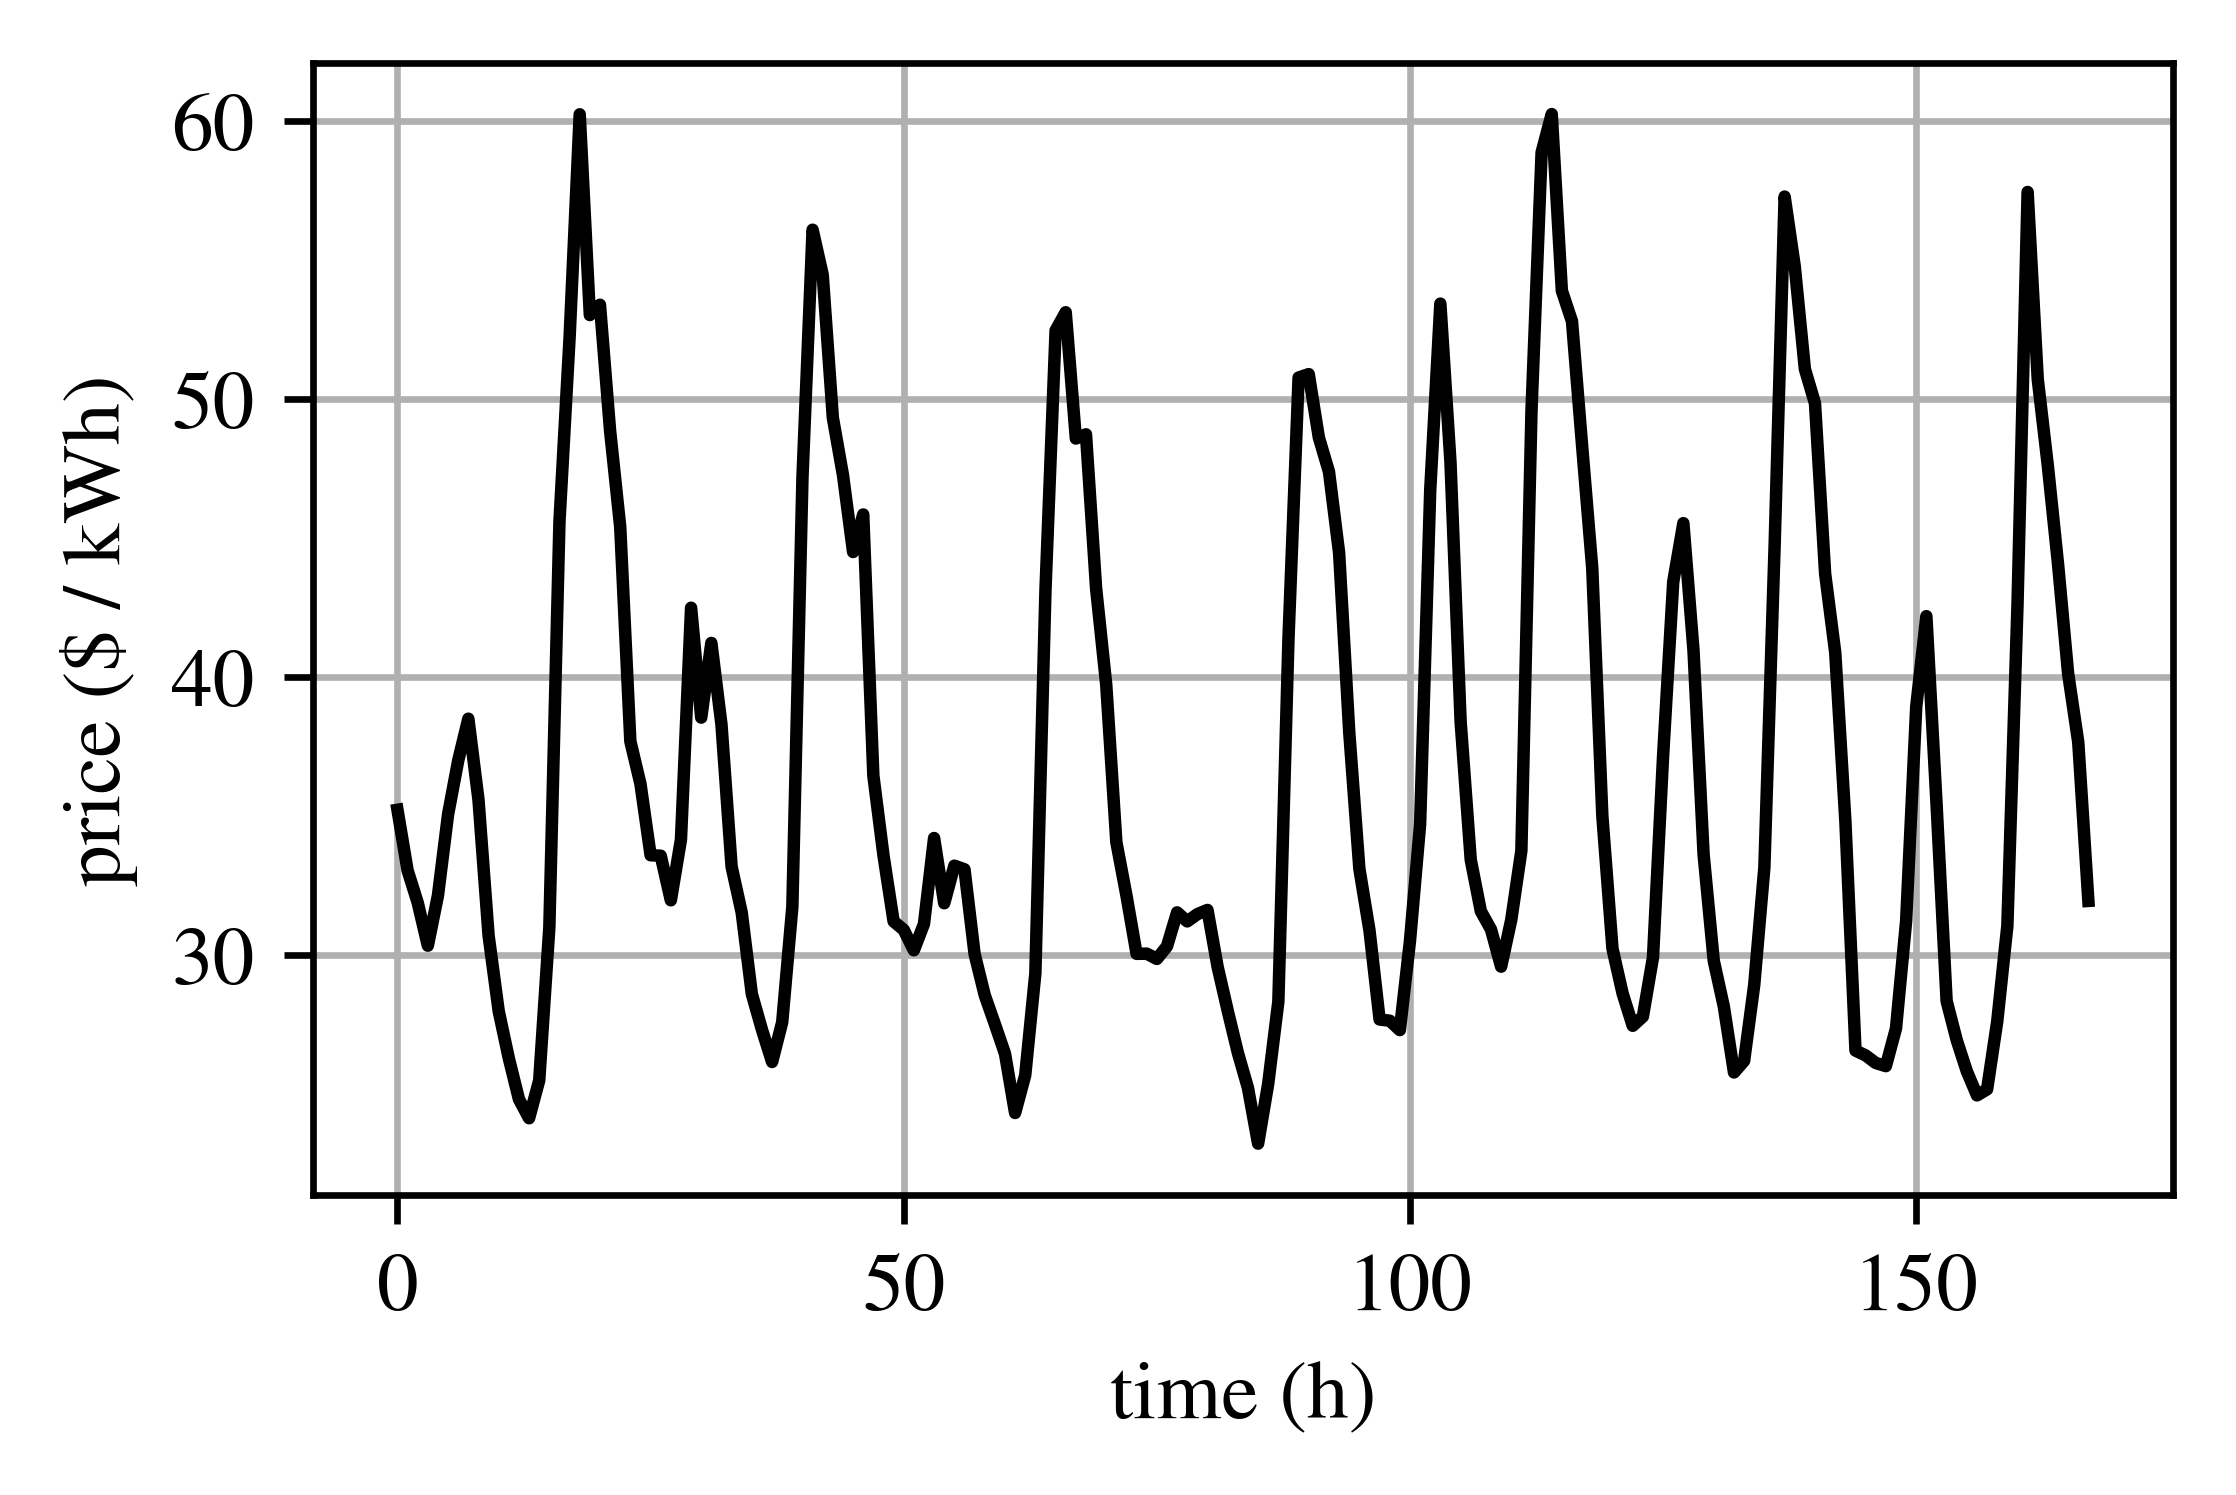
\includegraphics[width=0.45\textwidth]{fig_1.png}
\caption{An example of time series behavior observed in the CAISO from January 1st, 2015 to January 7th, 2015.}
\label{fig:ex_prices}
\end{figure}

Many standard time series forecasting methods have been used to predict DAM prices in the CAISO and other energy markets across the globe. For example, standard autoregressive integrated moving average (ARIMA) forecasting methods have been used to differing degrees of success in the CAISO market and the Spanish DAM. Conejo et al. have used ARIMA models to predict prices in the Spanish market with a 10\% error for the 2002 market \cite{Conejo2005a}. Furthermore, ARIMA has been shown to generate forecasts in the 2000 CAISO DAM with an error of around 13\% \cite{Garcia2005}. Another standard method for time series forecasting that has been used in the  Generalized autoregressive conditional heteroskedasticity (GARCH) method. Similar to ARIMA models, an error rate of around 10\% for the Spanish DAM has been reported when using GARCH \cite{Garcia2005}. More advanced hybrid methods have also been used for DAM forecasting. These methods include the usage of wavelet decompositions in order remove noise from data as well as the incorporation of ARIMA models in conjunction with GARCH methods \cite{Conejo2005,Tan2010,Amjady2008,Wang2012}. These various hybrid methods have error rates reported that range from as low as 1\% to as high as 25\%. 

%\cite{Conejo2005,Tan2010,Shafie-khah2011,Amjady2008}.

Recent advances in Recurrent Neural Networks (RNN) in the past 5 to 10 years have motivated this project to investigate their potential ability to predict CAISO DAM prices. The remainder of the paper will be organized in the following manner.

\begin{itemize}
	\item Section \ref{sec:approach}: A problem statement along with the design of the RNN, an explanation of the dataset, and software implementation details.
	\item Section \ref{sec:results}: Results of the forecasting performance of our RNN forecaster is presented.
	\item Section \ref{sec:discussion}: A discussion of how RNN forecasting compares to existing methods and other insights from this project.
	\item Section \ref{sec:conclusions}: Major findings from the paper are summarized.
\end{itemize}

% ============================================================================================================================= %
%														Approach																       %
% ============================================================================================================================= %

%\section{Approach}
%Because the dataset contains sequential information in the form of energy prices at different time increments, a recurrent neural network would be well suited to predicting future prices for this problem. This is because unlike in traditional neural networks, in recurrent neural networks there are loops that allow information about previous inputs to persist. In other words, it can use its memory from a previous time step to make a decision in a future time step. This is essential when working with time series data where order and contextual information is extremely important for accuracy.
%At a high level, the proposed model would utilize long short-term memory recurrent neural network architecture. Long short-term memory networks are ideal for making time series predictions because they allow the model to decide what information to keep and what information to forget. This allows them to deal with gaps of unknown duration between notable events in a time series.
%Our network will accept an input vector of past time series values and then return an output vector of predicted prices over the next 48 hours. 

\section{Modeling Approach}
\label{sec:approach}

\subsection{Problem Statement}

INCLUDE HOW ERROR IS CALCULATED!

\subsection{Neural Network Methodology}

Outline:
\begin{itemize}
	\item Basic explanation of an RNN.
	\item How does an RNN relate to energy prices.
	\item Figure: How does our RNN look in relation to energy prices.
	\item What are the specifics of the RNN we use.
	\item What was the methodology we used to determine the this design.
\end{itemize}

\subsection{Data Sources}
The dataset for this project was kindly provided by the Dowling Lab for Uncertainty Quantification and Mathematical Optimization at the University of Notre Dame in the Department of Chemical and Biomolecular Engineering. The dataset is comprised of over 6500 energy vendors, called nodes, participating in the CAISO. There is a full year's worth of data for each node in 2015, and price measurements are recorded at 1 hour intervals. Latitude and longitude coordinates are known for around 2000 of these nodes for visualization purposes. However, because of the limited timeline of this project, only 50 of these nodes will be used, and only a single week of data in January 2015 will be used for testing purposes. This is a reasonable thing to do as many papers report error values for single weeks in Janurary \cite{Conejo2005a,Garcia2005,Tan2010}. Furthermore, these papers only report results for single nodes in the DAM. Because our results include 50 nodes, it can be concluded that the results obtained for this dataset are statistically significant. 

\subsection{Software Implementation}

Outline:
\begin{itemize}
	\item Tensorflow
	\item CRC GPUs
	\item Code available at: GitHub
\end{itemize}


% ============================================================================================================================= %
%														Results																       %
% ============================================================================================================================= %
\section{Results}
\label{sec:results}

Figures and Tables we will need:
\begin{itemize}
	\item Figure: Example of what a price forecast looks like (good and bad).
	\item Figure: Histogram of error values for all nodes.
	\item Figure: Histogram of what adding more training data does for testing.
	\item Figure: Histogram of error values for the single node across the whole year.
	\item Table: Aggregated statistics of all nodes with low and high amounts of training.
	\item Table: Aggregated statistics of single node across the year.
	\item Table: Aggregated statistics on CPU time.
\end{itemize}

\begin{figure}[h]
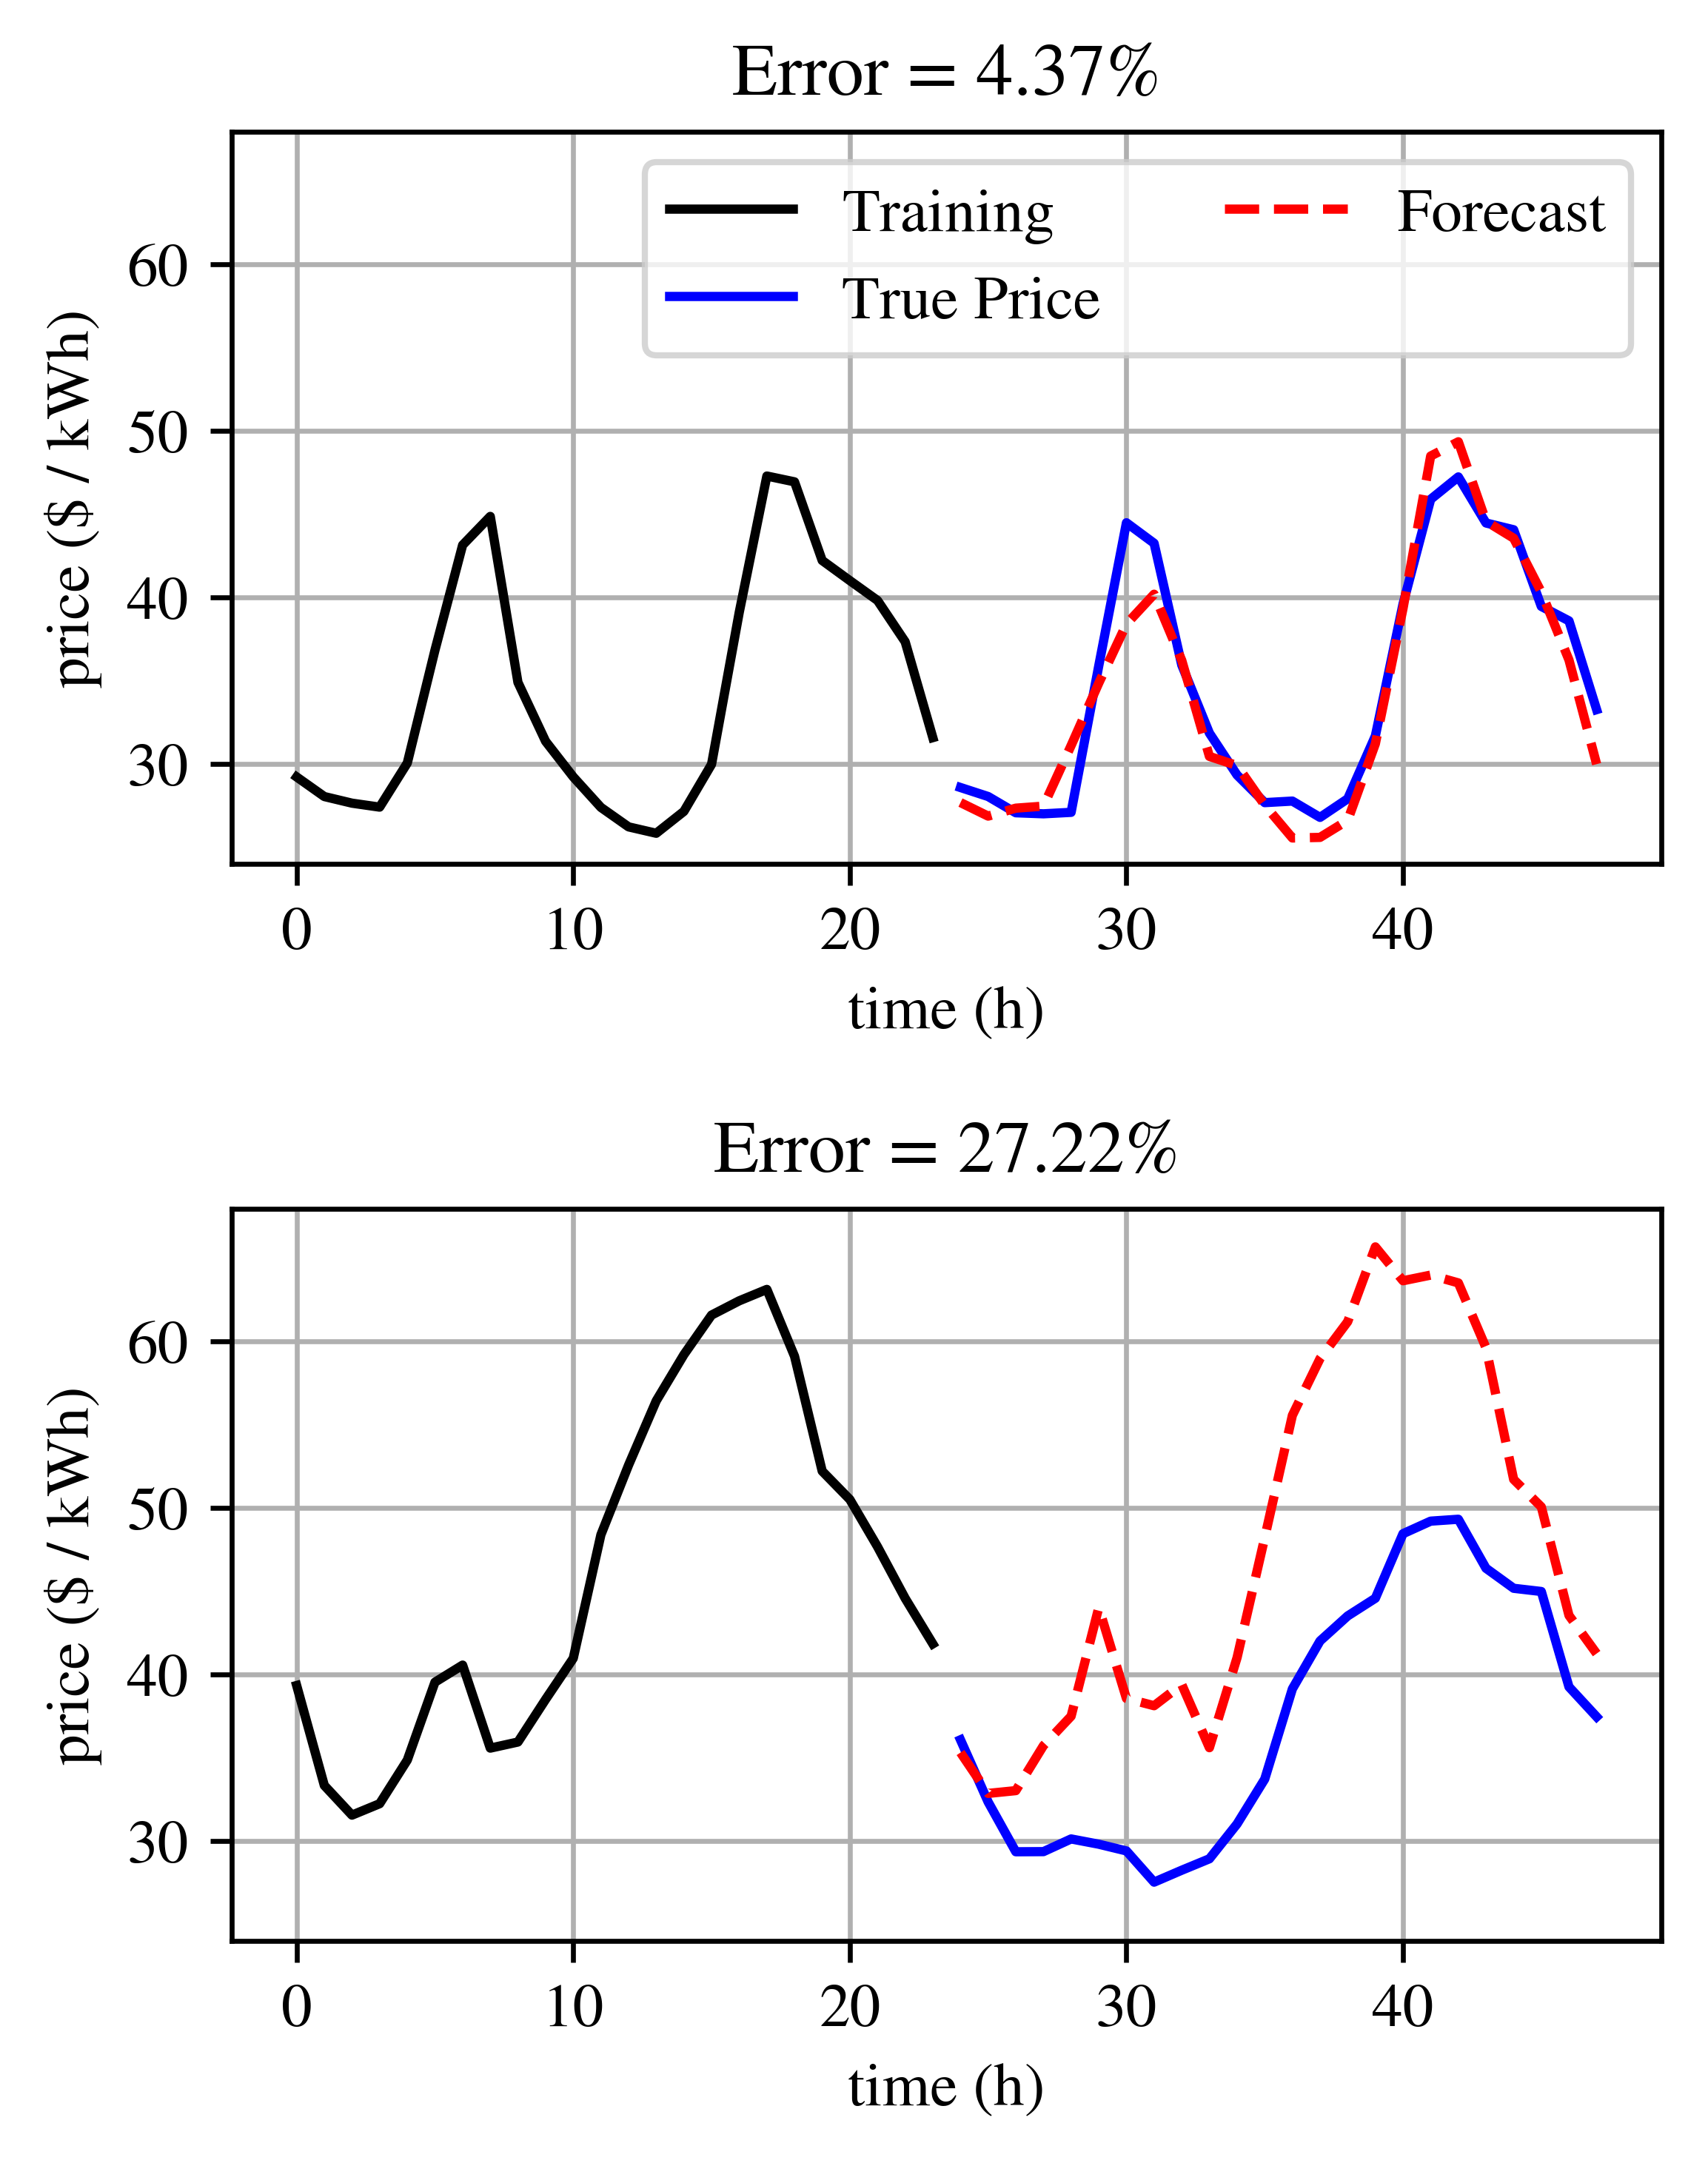
\includegraphics[width=0.45\textwidth]{fig_3.png}
\caption{Example price forecasting using our RNN.}
\label{fig:ex_prices}
\end{figure}

\begin{figure}[h]
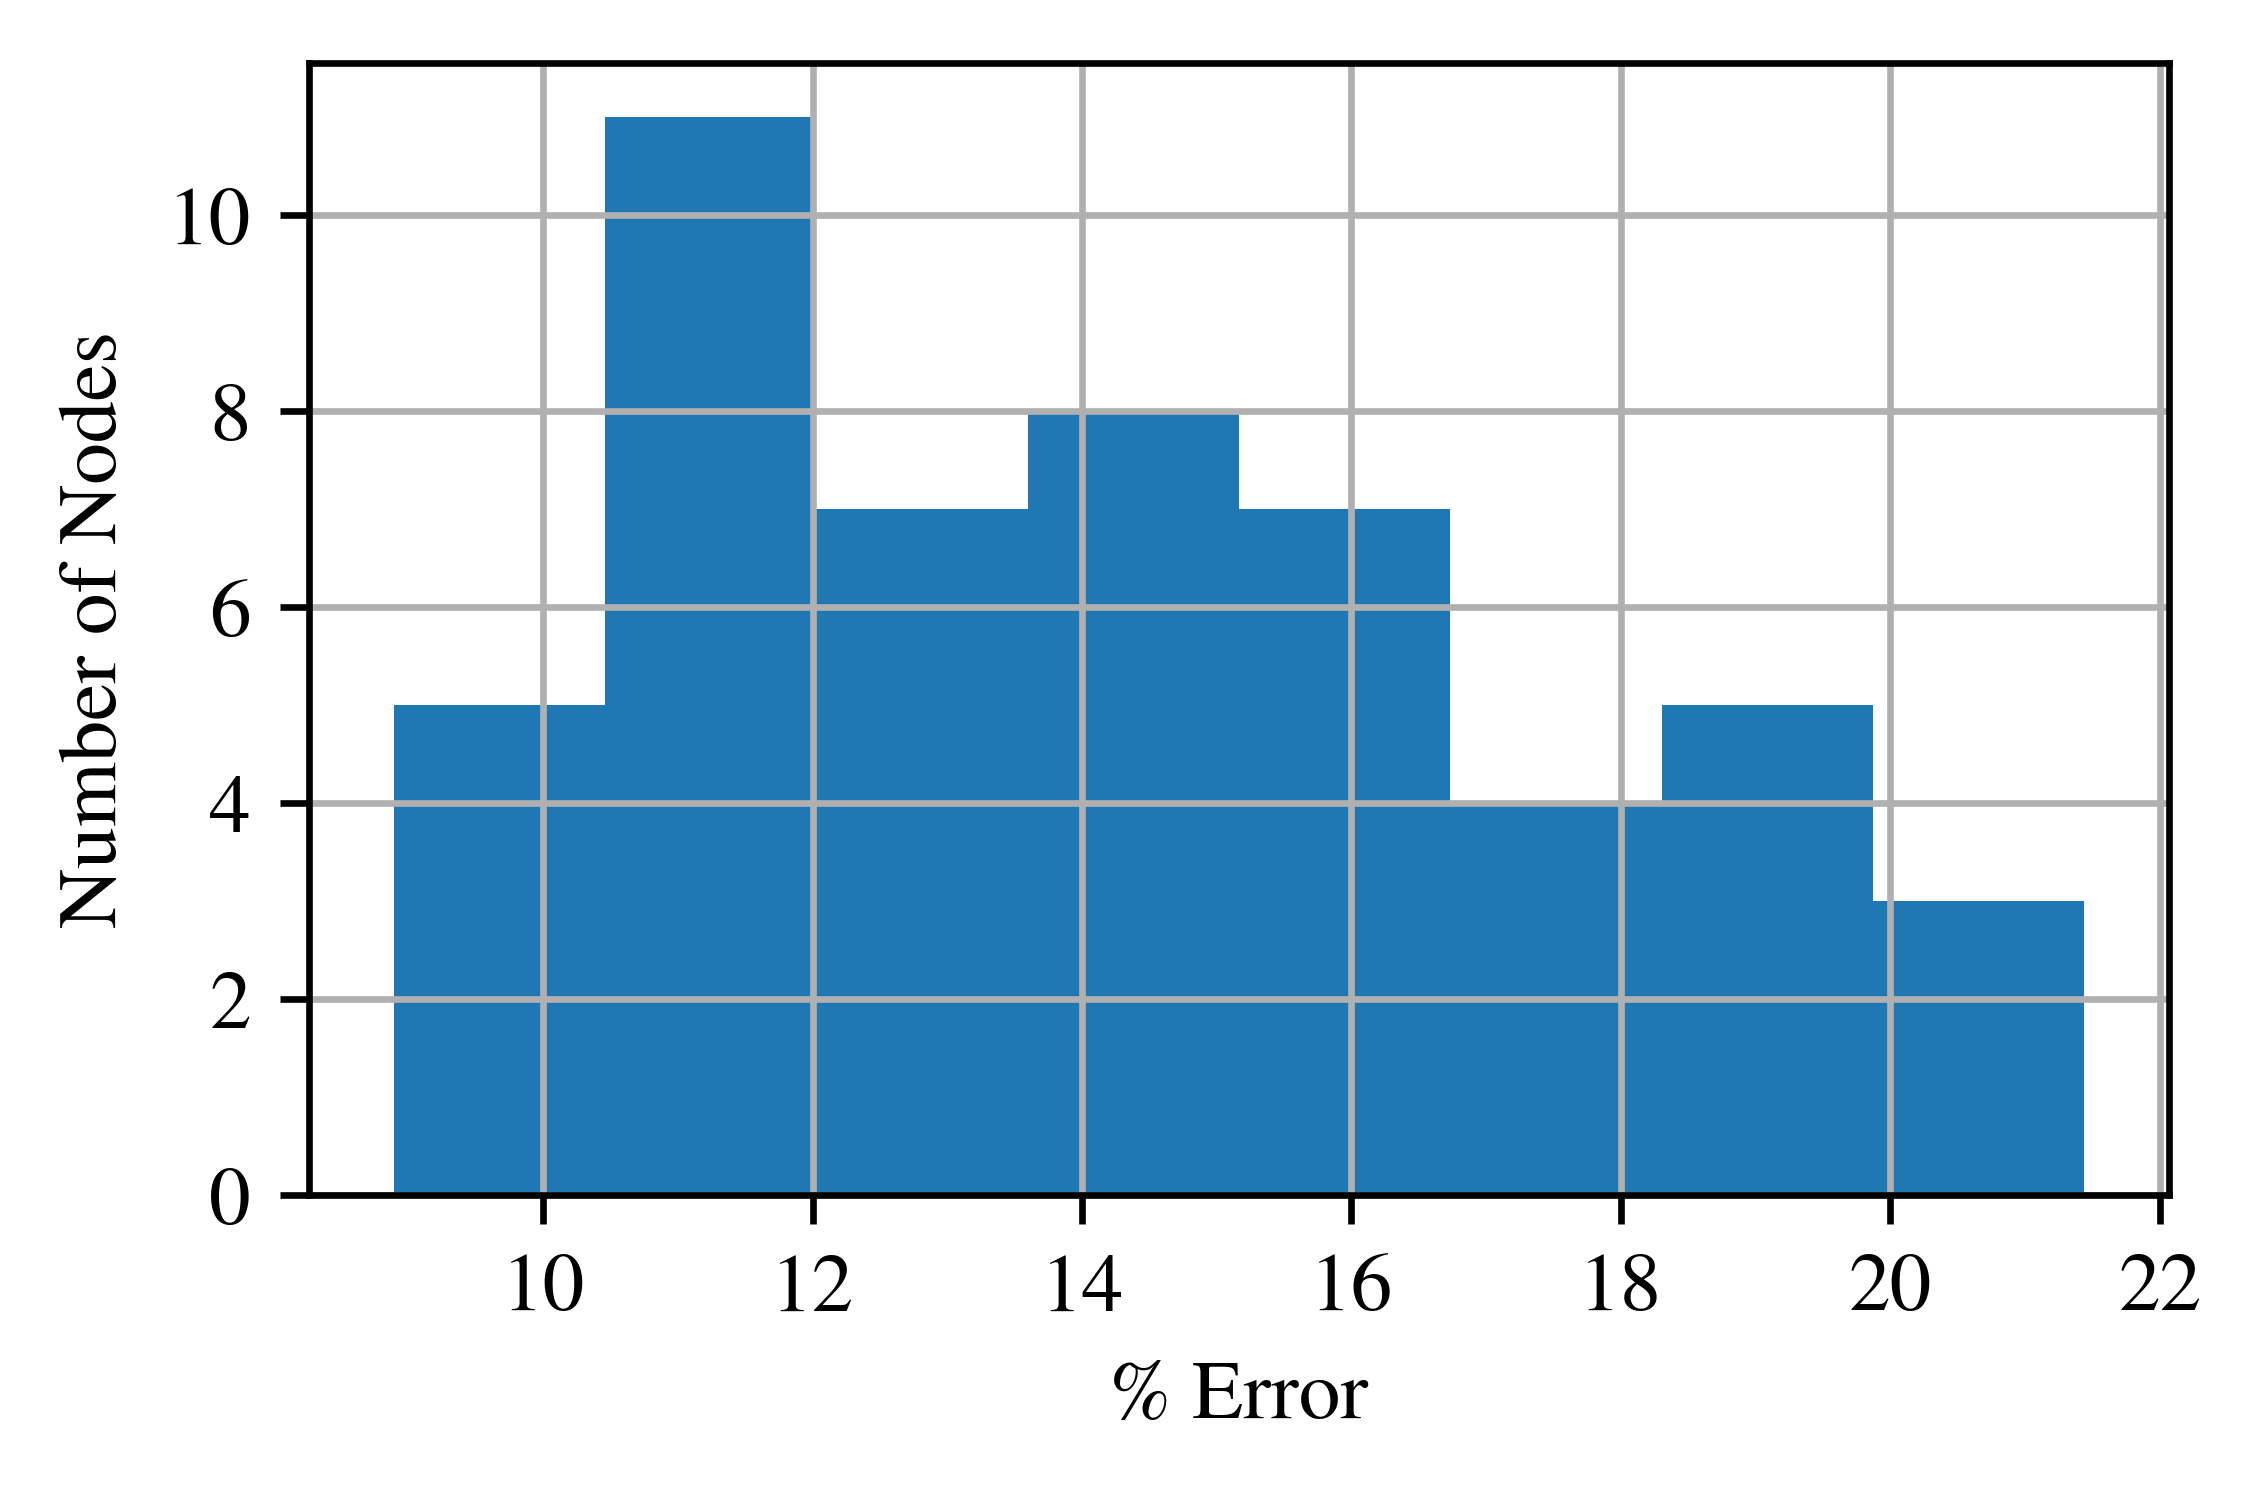
\includegraphics[width=0.45\textwidth]{fig_5.png}
\caption{Histogram of all nodes.}
\label{fig:hist_small}
\end{figure}

% Still running on CRC

%\begin{figure}[h]
%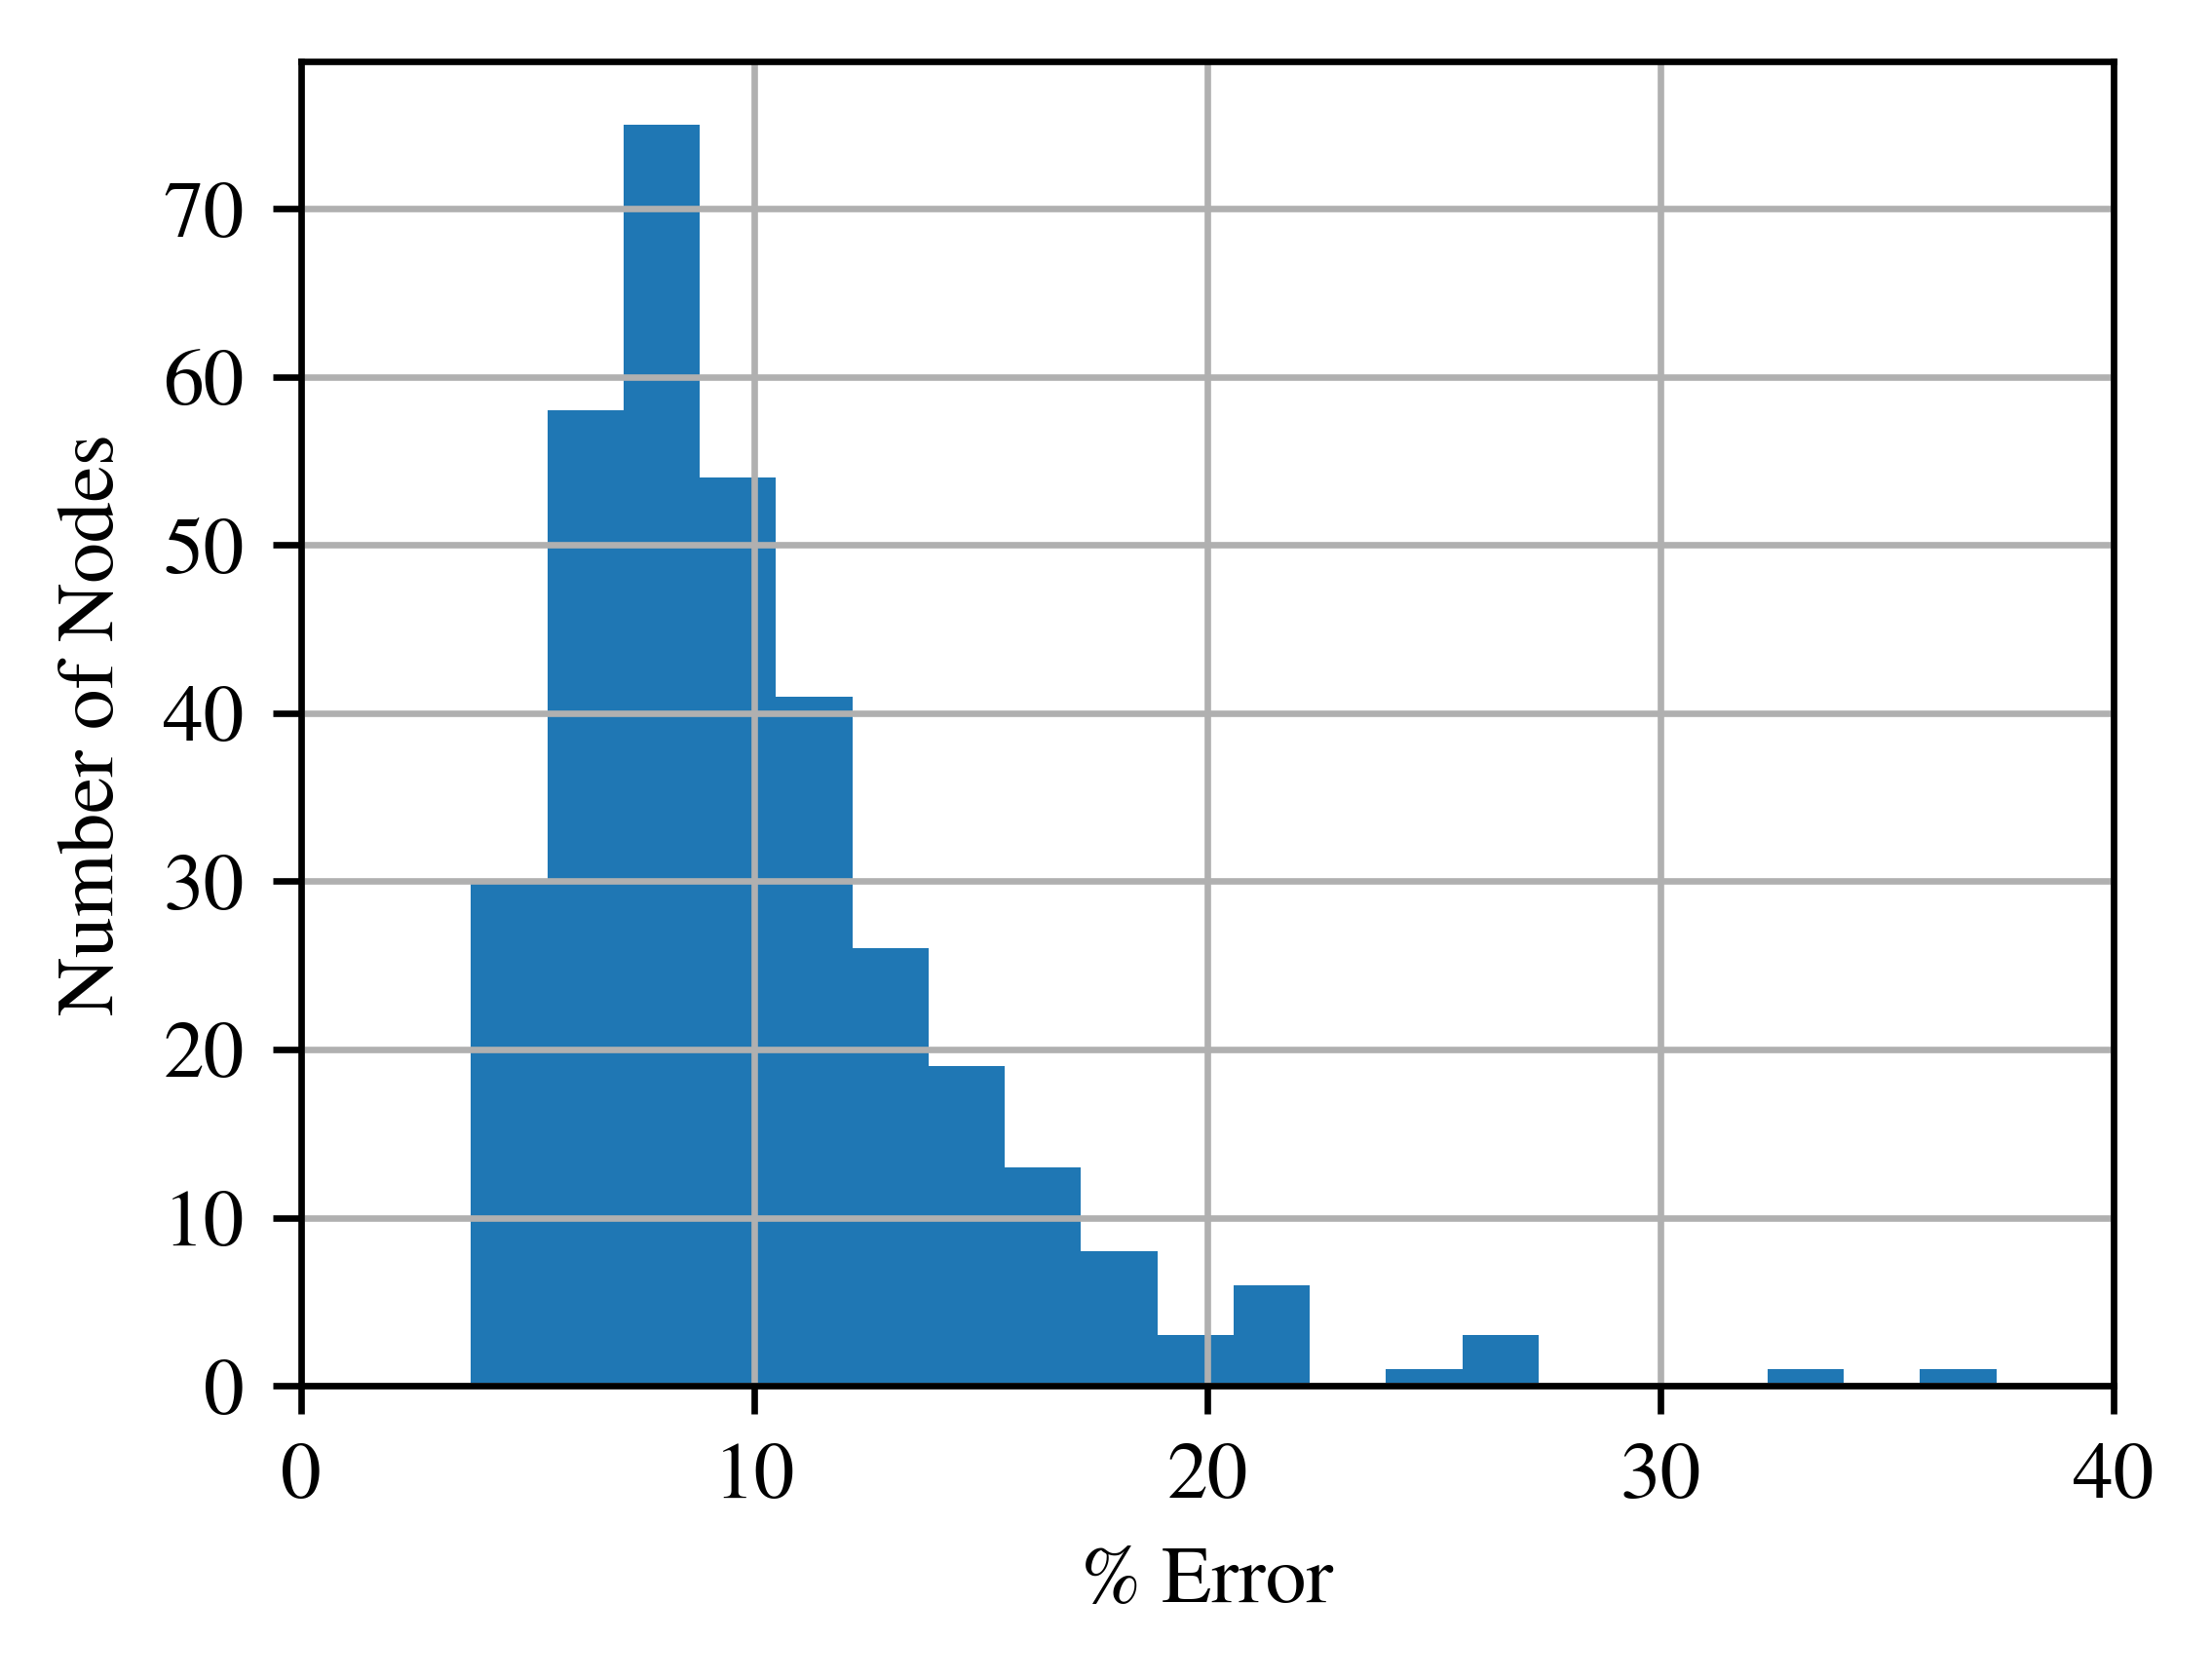
\includegraphics[width=0.45\textwidth]{fig_6.png}
%\caption{Histogram of all nodes now with larger amounts of training data.}
%\label{fig:hist_large}
%\end{figure}

\begin{figure}[h]
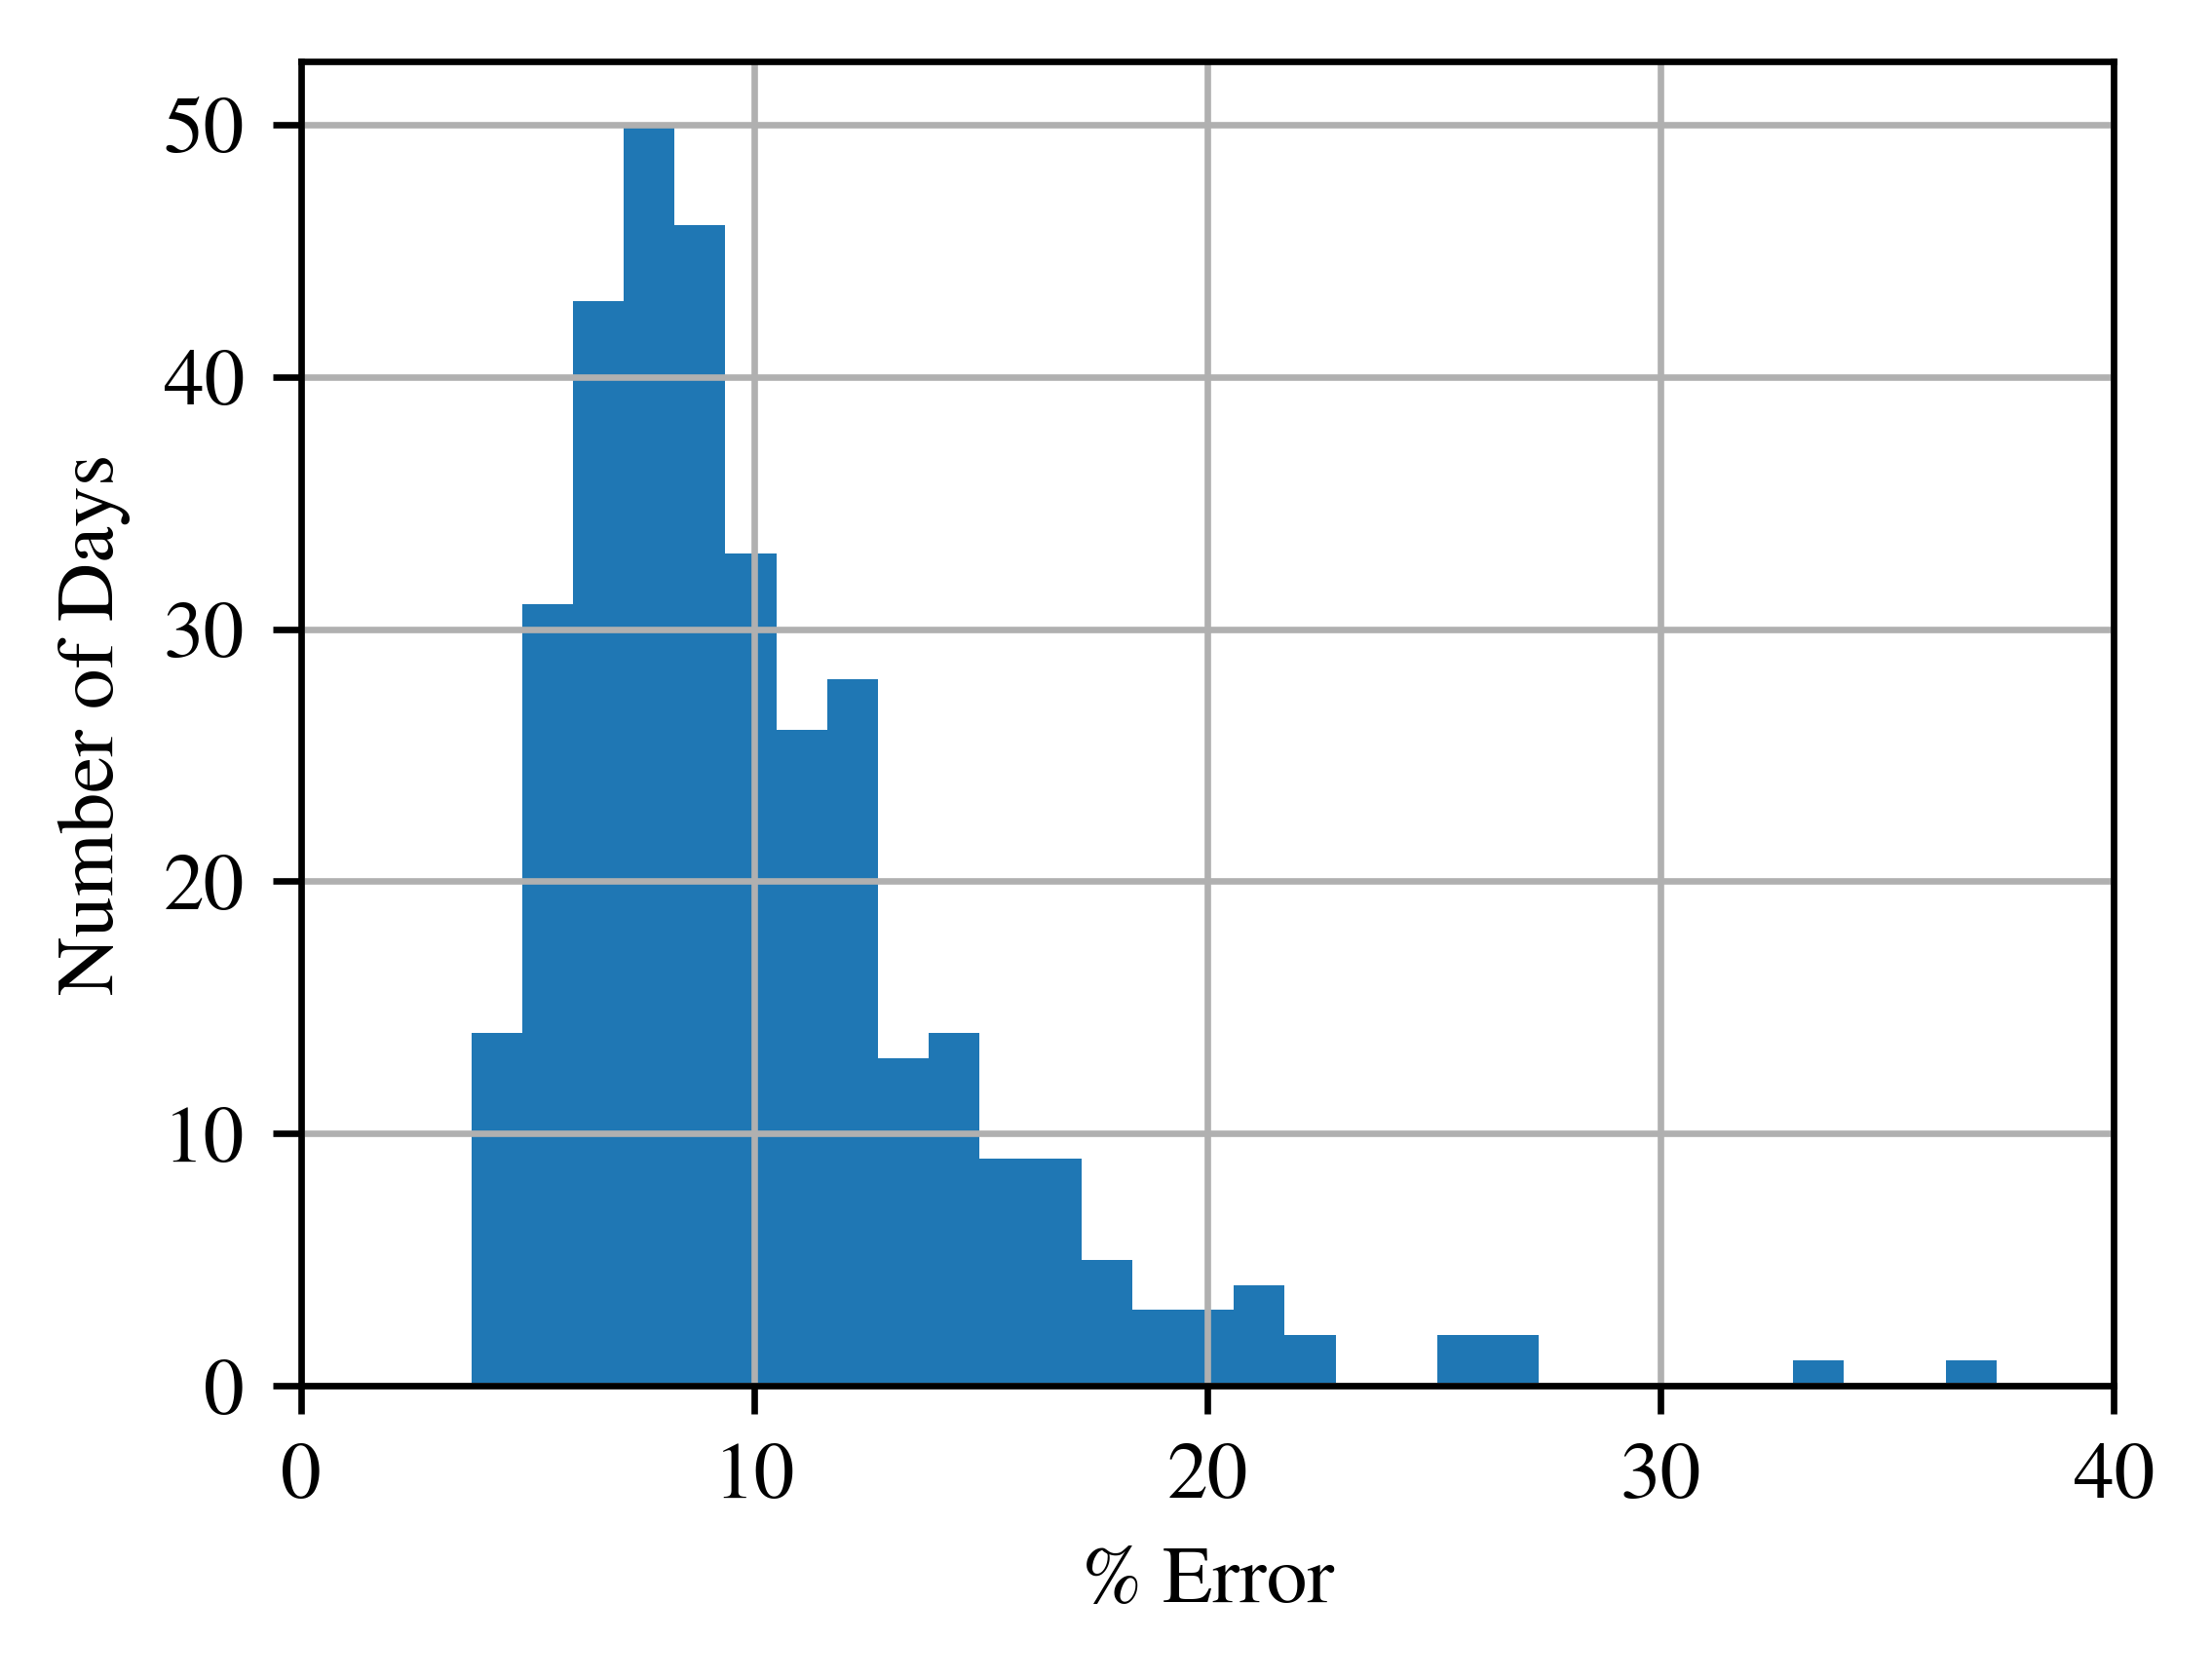
\includegraphics[width=0.45\textwidth]{fig_7.png}
\caption{Histogram of a single node run through the whole year.}
\label{fig:hist_single}
\end{figure}

\begin{figure}[h]
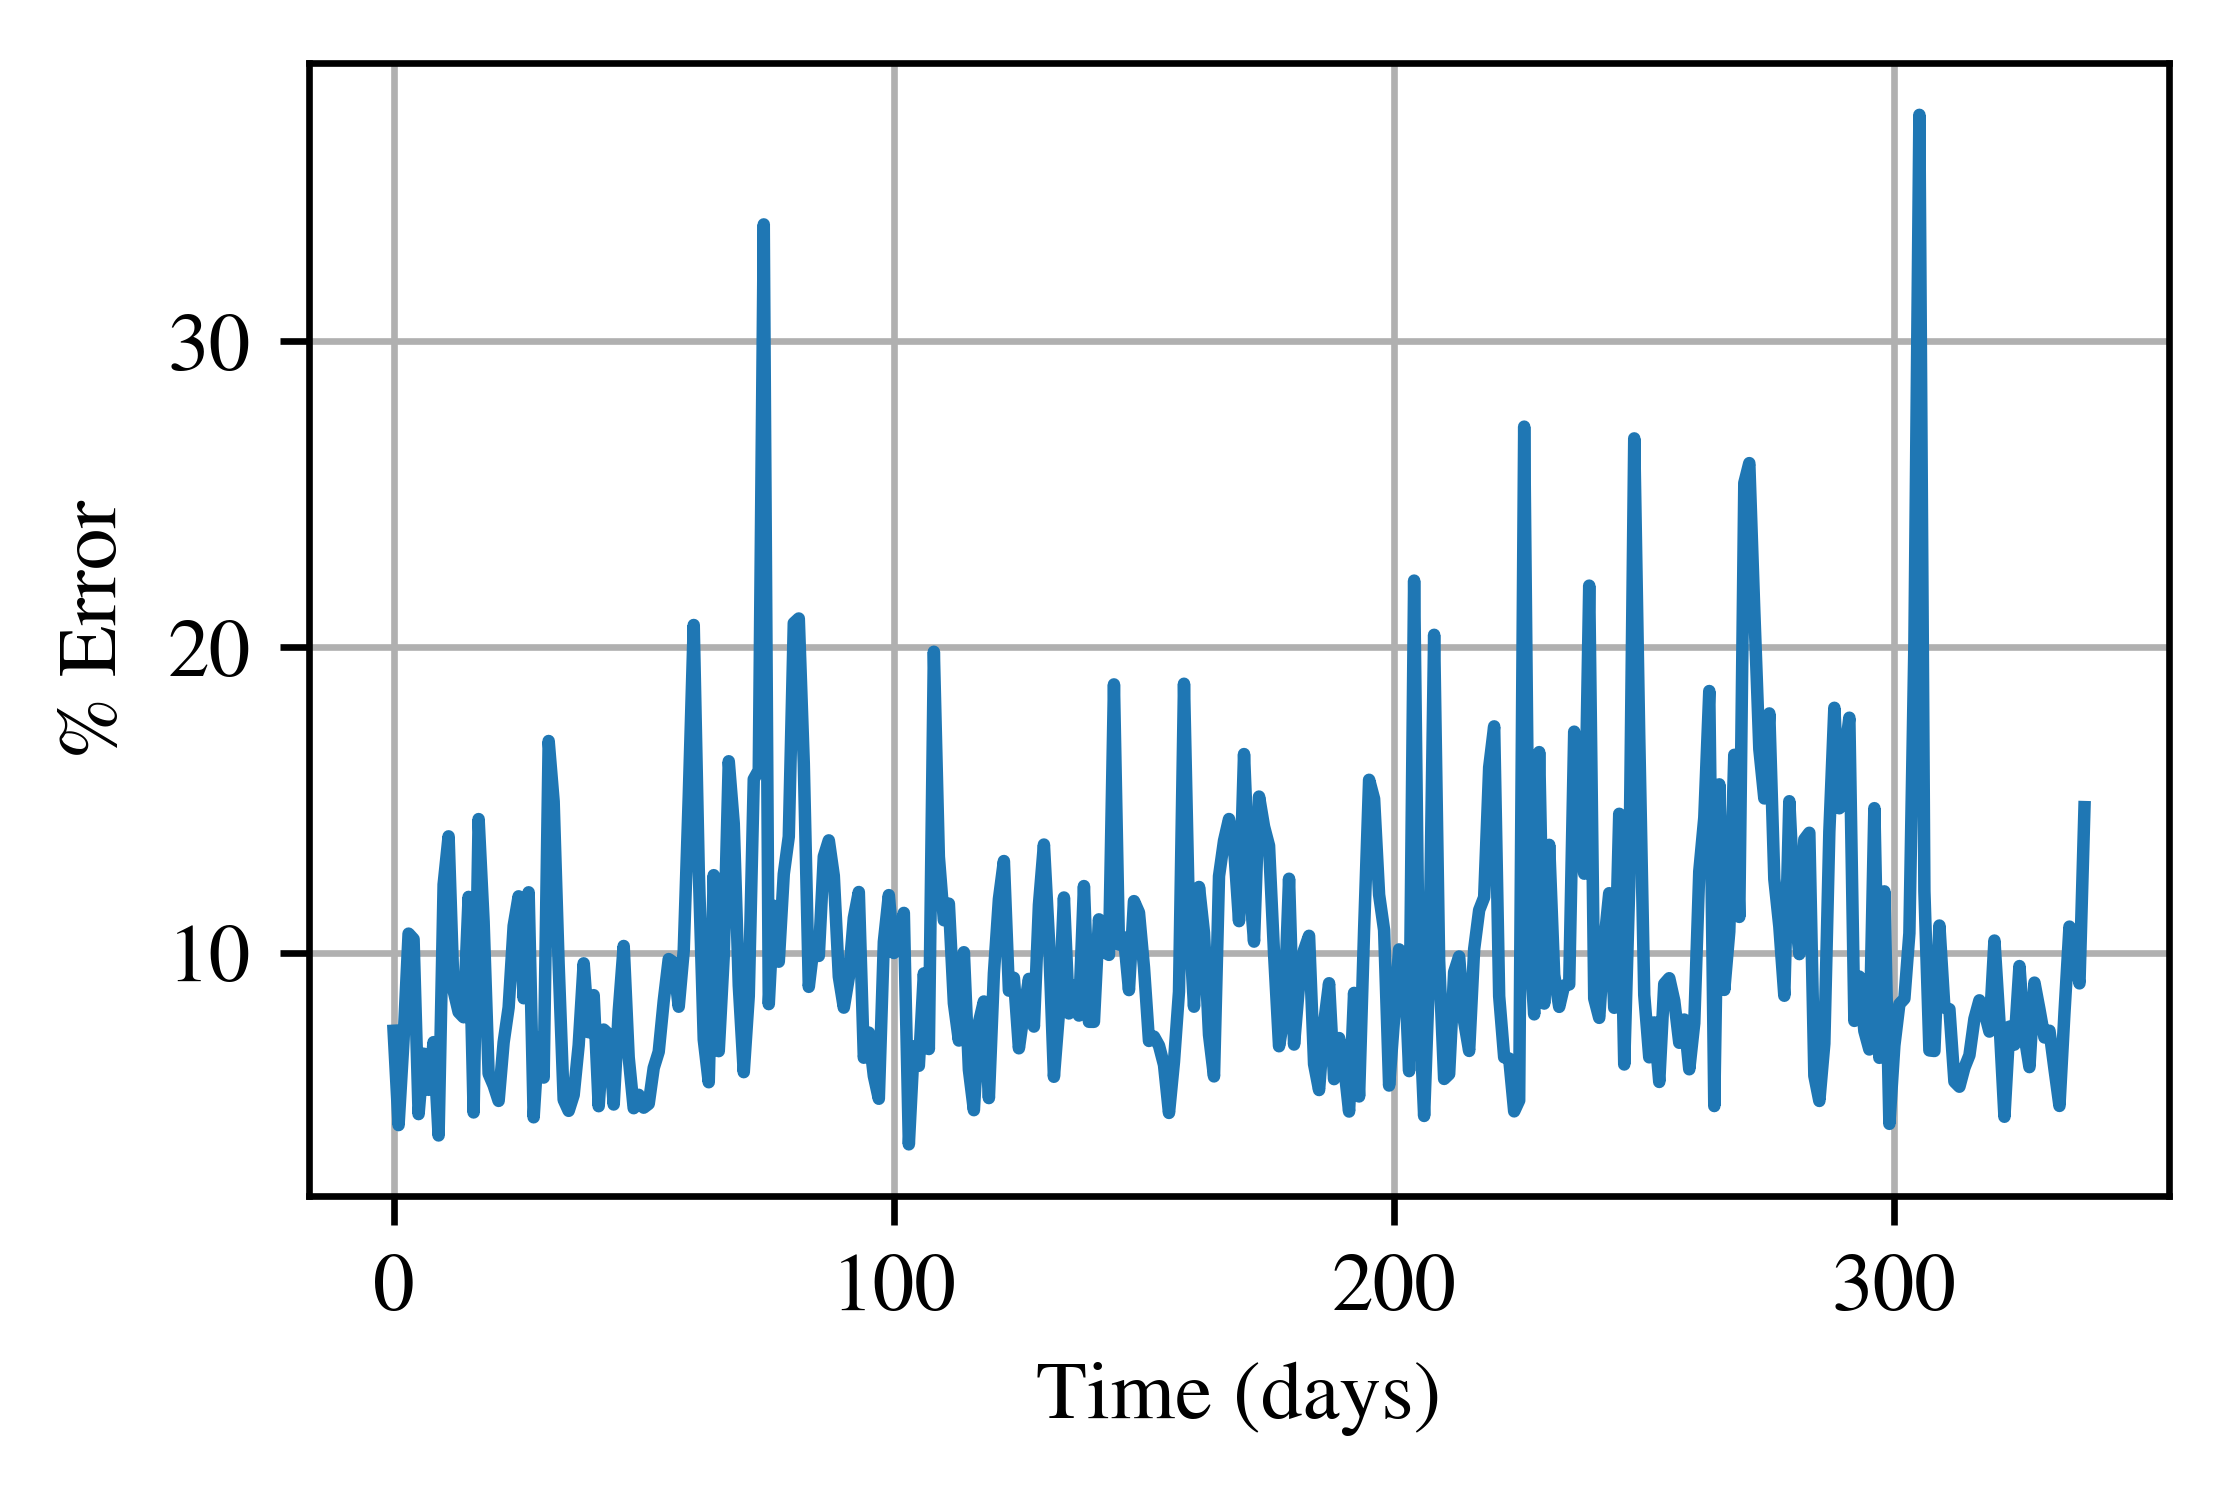
\includegraphics[width=0.45\textwidth]{fig_8.png}
\caption{Time series plot of a single node run through the whole year.}
\label{fig:time_single}
\end{figure}

% ============================================================================================================================= %
%														Discussion															       %
% ============================================================================================================================= %
\section{Discussion}
\label{sec:discussion}

Figures and Tables we will need:
\begin{itemize}
	\item Figure: Graphical comparison of how backcasting does not do what the RNN can do.
	\item Figure/Table: Comparison to techniques that have been mentioned earlier in the paper and backcasting.
\end{itemize}

% ============================================================================================================================= %
%														Conclusions															       %
% ============================================================================================================================= %
\section{Conclusions and Future Work}
\label{sec:conclusions}

% ============================================================================================================================= %
%														References															       %
% ============================================================================================================================= %

%\section{Related Work}
%\begin{itemize}
%    \item Here provide the relevant references for your work. 
%\end{itemize}
%	
%\emph{Use the standard Communications of the ACM format for references --- that is, a numbered list at the end of the article, ordered alphabetically by first author, and referenced by numbers in brackets~. See the examples of citations at the end of this document. Within this template file, use the style named references for the text of your citation.}
%
%\emph{References should be published materials accessible to the public. Internal technical reports may be cited only if they are easily accessible (i.e. you can give the address to obtain the report within your citation) and may be obtained by any reader. Proprietary information may not be cited. Private communications should be acknowledged, not referenced  (e.g., ``[Robertson, personal communication]").}


\bibliographystyle{ACM-Reference-Format}
%\bibliography{acmart.bib}
\bibliography{/Users/ClayElmore/Desktop/mendeley/DMD_Literature.bib}
\end{document}
